% This is "sig-alternate.tex" V2.0 May 2012
% This file should be compiled with V2.5 of "sig-alternate.cls" May 2012
%
% This example file demonstrates the use of the 'sig-alternate.cls'
% V2.5 LaTeX2e document class file. It is for those submitting
% articles to ACM Conference Proceedings WHO DO NOT WISH TO
% STRICTLY ADHERE TO THE SIGS (PUBS-BOARD-ENDORSED) STYLE.
% The 'sig-alternate.cls' file will produce a similar-looking,
% albeit, 'tighter' paper resulting in, invariably, fewer pages.
%
% ----------------------------------------------------------------------------------------------------------------
% This .tex file (and associated .cls V2.5) produces:
%       1) The Permission Statement
%       2) The Conference (location) Info information
%       3) The Copyright Line with ACM data
%       4) NO page numbers
%
% as against the acm_proc_article-sp.cls file which
% DOES NOT produce 1) thru' 3) above.
%
% Using 'sig-alternate.cls' you have control, however, from within
% the source .tex file, over both the CopyrightYear
% (defaulted to 200X) and the ACM Copyright Data
% (defaulted to X-XXXXX-XX-X/XX/XX).
% e.g.
% \CopyrightYear{2007} will cause 2007 to appear in the copyright line.
% \crdata{0-12345-67-8/90/12} will cause 0-12345-67-8/90/12 to appear in the copyright line.
%
% ---------------------------------------------------------------------------------------------------------------
% This .tex source is an example which *does* use
% the .bib file (from which the .bbl file % is produced).
% REMEMBER HOWEVER: After having produced the .bbl file,
% and prior to final submission, you *NEED* to 'insert'
% your .bbl file into your source .tex file so as to provide
% ONE 'self-contained' source file.
%
% ================= IF YOU HAVE QUESTIONS =======================
% Questions regarding the SIGS styles, SIGS policies and
% procedures, Conferences etc. should be sent to
% Adrienne Griscti (griscti@acm.org)
%
% Technical questions _only_ to
% Gerald Murray (murray@hq.acm.org)
% ===============================================================
%
% For tracking purposes - this is V2.0 - May 2012

\documentclass{sig-alternate}

\setlength{\paperheight}{11in}
\setlength{\paperwidth}{8.5in}
\usepackage[
  pass,% keep layout unchanged 
  % showframe,% show the layout
]{geometry}

\usepackage{listings}
\usepackage{url}

\pdfpagewidth=8.5in
\pdfpageheight=11in


\begin{document}

\clubpenalty=10000
\widowpenalty=10000


\newfont{\mycrnotice}{ptmr8t at 7pt}
\newfont{\myconfname}{ptmri8t at 7pt}
\let\crnotice\mycrnotice%
\let\confname\myconfname%

\permission{Permission to make digital or hard copies of part or all of this work for personal or classroom use is granted without fee provided that copies are not made or distributed for profit or commercial advantage, and that copies bear this notice and the full citation on the first page. Copyrights for third-party components of this work must be honored. For all other uses, contact the Owner/Author.\\ Copyright is held by the owner/author(s).}
\conferenceinfo{DEBS'15,} {June 29 - July 3, 2015, OSLO, Norway.}
\copyrightetc{ACM \the\acmcopyr}
\crdata{978-1-4503-3286-6/15/06\ ...\$15.00.\\
http://dx.doi.org/10.1145/2675743.2774214}



%
% --- Author Metadata here ---
%\conferenceinfo{DEBS`14} {May 26-29, 2014,Mumbai,India.}\CopyrightYear{2014}
%\crdata{978-1-4503-2737-4/14/05\ …\$15.00.\\
 %}
\clubpenalty=10000

\widowpenalty = 10000

%\CopyrightYear{2007} % Allows default copyright year (20XX) to be over-ridden - IF NEED BE.
%\crdata{0-12345-67-8/90/01}  % Allows default copyright data (0-89791-88-6/97/05) to be over-ridden - IF NEED BE.
% --- End of Author Metadata ---

\title{Tutorial: Solution Patterns for Realtime Streaming Analytics}

\lstdefinelanguage{siddhi}
{morekeywords={from, select, insert into, define}
sensitive=false,
morecomment=[l]{//},
morecomment=[s]{/*}{*/},
morestring=[b]",
morestring=[d]'
}


\lstset{tabsize=2}
\lstset{basicstyle=\scriptsize\ttfamily}
%\lstset{numbers=left, numberstyle=\tiny, stepnumber=1,numbersep=2pt,firstnumber=1}
\lstset{frame=tb}
%
% You need the command \numberofauthors to handle the 'placement
% and alignment' of the authors beneath the title.
%
% For aesthetic reasons, we recommend 'three authors at a time'
% i.e. three 'name/affiliation blocks' be placed beneath the title.
%
% NOTE: You are NOT restricted in how many 'rows' of
% "name/affiliations" may appear. We just ask that you restrict
% the number of 'columns' to three.
%
% Because of the available 'opening page real-estate'
% we ask you to refrain from putting more than six authors
% (two rows with three columns) beneath the article title.
% More than six makes the first-page appear very cluttered indeed.
%
% Use the \alignauthor commands to handle the names
% and affiliations for an 'aesthetic maximum' of six authors.
% Add names, affiliations, addresses for
% the seventh etc. author(s) as the argument for the
% \additionalauthors command.
% These 'additional authors' will be output/set for you
% without further effort on your part as the last section in
% the body of your article BEFORE References or any Appendices.

\numberofauthors{1} %  in this sample file, there are a *total*
% of EIGHT authors. SIX appear on the 'first-page' (for formatting
% reasons) and the remaining two appear in the \additionalauthors section.
%
% There's nothing stopping you putting the seventh, eighth, etc.
% author on the opening page (as the 'third row') but we ask,
% for aesthetic reasons that you place these 'additional authors'
% in the \additional authors block, viz.


\author{
% You can go ahead and credit any number of authors here,
% e.g. one 'row of three' or two rows (consisting of one row of three
% and a second row of one, two or three).
%
% The command \alignauthor (no curly braces needed) should
% precede each author name, affiliation/snail-mail address and
% e-mail address. Additionally, tag each line of
% affiliation/address with \affaddr, and tag the
% e-mail address with \email.
%
% 1st. author
\alignauthor
Srinath Perera, Suhothayan Sriskandarajah\\
       \affaddr{WSO2 Inc.}\\
       \affaddr{Mountain View, CA, USA}\\
       \email{\{srinath, suho \}@wso2.com}
}

\maketitle
\begin{abstract}
Large-scale data analytics has received much attention under the theme ``Big Data". Big data usecases have found a wide range of applications from individual health monitoring to urban planning. Even at this initial stages, big data has demonstrated it's potential to transform the world. Although most early usecases used batch processing technologies like MapReduce, there are many usecases such as stock markets, traffic, surveillance, and patient monitoring that need realtime analytics. Realtime Analytics Technologies like Apache Storm, Spark Streaming, and several Complex Event Processing systems have received attention under realtime analytics. However, most practitioners still focus on implementing realtime analytics from the scratch. There is no common shared understanding about how to implement those analytics usecases among the early adopters. This tutorial tries to address this gap by describing thirteen common relatime analytics patterns and explaining how to implement them. In the discussion, we will draw heavily from real life usecases done under Complex Event Processing and other technologies. 
\end{abstract}

% A category with the (minimum) three required fields
\category{C.2.4}{Distributed Systems}{Distributed applications}
%A category including the fourth, optional field follows..
\category{I.5}{Pattern Recognition}{Implementation}

\terms{Performance, Design}

\keywords{Complex Event Processing, Events, Data Processing}



\section{Introduction}

Google's MapReduce paper published in 2005 introduced a simple and scalable data processing technique that can be used with commodity hardware. Since then, Data Analytics--processing data and deriving actionable insights from data--has received much attention from both the Industry and the Academia.  Most initial use cases were batch analytics, which stored data in a disk and then periodically processes data by walking through it. Unless data is small, batch analytics would take minutes to produce an output. However, for some use cases ( e.g., stock markets, traffic, surveillance, and patient monitoring), the value of insights degrades very quickly with time. For an example, analytics from stock markets are often useless within milliseconds. Batch processing technologies like MapReduce, which take from minutes to hours to produce an output, are not suitable for such use cases. To fill that gap, architects have adopted technologies like In-Memory Computing (VoltDB~\cite{voltdb}, ZAP Hana~\cite{saphana}), Stream Processing (e.g., Apache Storm~\cite{storm}, Apache Samza~\cite{samza}), and Complex Event Processing (Esper~\cite{esper}, WSO2 CEP~\cite{siddhi}, Tibco StreamBase~\cite{streambase}).

Realtime analytics uses cases have two flavors.  

\begin{enumerate}
\item Realtime Interactive/Ad-hoc Analytics - users issue ad-hoc dynamic queries and the system responds interactively. Among the examples of such systems are Druid, SAP Hana, VoltDB, MemSQL, and Apache Drill. 
\item Realtime Streaming Analytics - users issue static queries once and they do not change. The system process data as they come in without storing). CEP and Stream Processing technologies are two example technologies that enable streaming analytics. 
\end{enumerate}

Realtime Interactive Analytics allows users to explore a large data set by issuing interactive queries. They should respond within 10 seconds, which is considered the upper bound for acceptable human interaction. In contrast, this tutorial focuses on Realtime Streaming Analytics, which is processing data and reacting to them very fast as they come in, often within few milliseconds. Such technologies are not new. History goes back to Active Databases (2000+), Stream processing (e.g. Aurora~\cite{abadi_aurora:_2003}, Borealis~\cite{abadi_design_2005} (2005+) and later Apache Storm), Distributed Streaming Operators as a Database research topic around 2005, and Complex Event processing (see \cite{marketSurvey}).

Still when thinking about realtime analytics, many think only counting use cases. As we shall discuss, counting use cases are only the tip of the iceberg of real life realtime use cases. Since the input data arrives as a data stream, a time dimension always presents in the data. This time dimension allows us to implement and perform much powerful use cases.  

Under the theme large scale streaming analytics, stream processing technologies like Apache Samza and Apache Storm have received much attention. However, these tools force every programmer to design and implement realtime analytics processing from first principles. For an example, if users need a time window, they need to implement it from first principles.  This is like every programmer implementing his own list data structure. Better understanding of common patterns will let us understand the domain better and build tools that handle those scenarios. This tutorial tries to address this gap by describing thirteen common relatime streaming analytics patterns and how to implement them. In the discussion, we will draw heavily from real life use cases done under Complex Event Processing and other technologies. 

The next section describes the patterns, and the following  section compares them against the patterns identified elsewhere. The fourth section describes pattern implementations. The final section concludes the discussion. 

\section{Realtime Stream Analytics Patterns}
 
Let's first agree on the terminology. Realtime Streaming Analytics accepts one or more data streams as input and produces one or more data streams as output. Each data stream consists of many events ordered in time. Each event has many attributes, but all events in a same stream have the same set of attributes or schema. One could think of data streams as a relational table that never ends where each event is a record in the table. 


\subsection{Pattern 1: Preprocessing}
Preprocessing is often done as a projection from one data stream to the other or through filtering. Potential operations include
\begin{enumerate}
\item Filtering some events
\item Reshaping a stream by removing, renaming, or adding new attributes to events in the stream
\item Splitting and combining attributes in a stream 
\item Transforming attributes   
\end{enumerate}

For example, from a twitter data stream, we might choose to extract the fields: author, timestamp, location, and then filter them based on the location of the author. 

\subsection{Pattern 2: Alerts and Thresholds}
This pattern detects a condition and generates alerts based on a condition. (e.g., Alarm on high temperature). These alerts can be based on a simple value or more complex conditions such as rate of increase etc. 

For an example, in a use case we implemented using transit data from London city, we trigger a speed alert  when a bus has exceeded a given speed limit. More details are described in TFL (Transport for London) Demo video \cite{tfl}. 
 
\begin{figure}[!htbp]
\centering
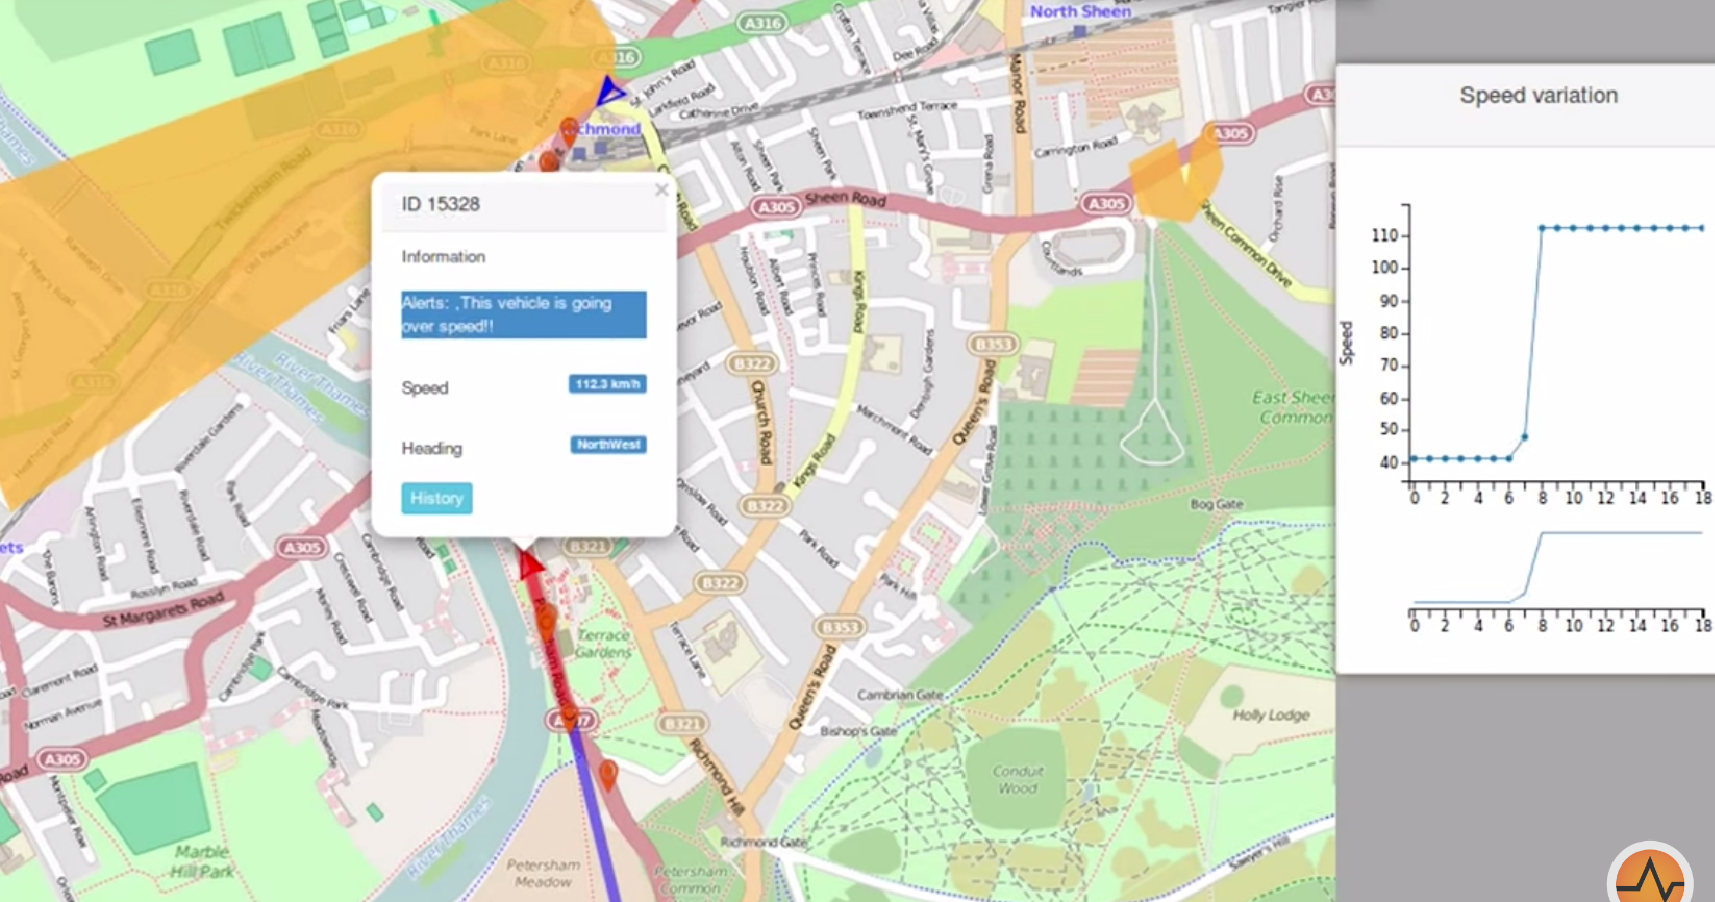
\epsfig{file=images/tfl.eps, height=1.5in}
\caption{TFL Demo}
\label{fig:q1}
\end{figure}

We can also generate alerts for more complex scenarios such as detecting if the server room temperature is continually increasing for the last five mins. 

\subsection{Pattern 3: Simple Counting and Counting with Windows}

This pattern includes aggregate functions like Min, Max, Percentiles, etc. They can be calculated without storing any data. (e.g., counting the number of failed transactions). 

However, counts are often useful with a time window attached to it.( e.g. failure count in the last hour). There are many types of windows: sliding windows vs. batch (tumbling) windows and time vs. length windows. There are four main variations. 

\begin{enumerate}
\item Time-sliding window: keeps each event for the given time window, produces an output whenever a new event has been added or removed. 
\item Time-batch window (called tumbling window): produces output at the end of the given time window
\item Length-sliding : same as the time-sliding window, but keeps a window of n events instead of selecting them by time.
\item Length-Batch window: same as the time-batch window, but keeps a window of n events instead of selecting them by time
\end{enumerate}

Also there are special windows like decaying windows and unique windows. 


\subsection{Pattern 4: Joining Event Streams}
Main idea behind this pattern is to combine multiple data streams and create a new event stream. For example, lets assume we play a football game where both the players and the ball having attached sensors that emit events that have current location and acceleration as properties. We can use ``joins" pattern to detect when a player has kicked the ball. We do that by joining the ball location stream and the player stream on the condition that they are close to each other by one meter and the ball's acceleration has increased by more than $55m/s^2$.

Among other use cases are combining data from two sensors, detecting collisions, and detecting proximity of two vehicles. 

\subsection{Pattern 5: Data Correlation, Missing Events, and Erroneous Data}

When we correlate events between different streams, we would use the forth pattern. In addition, we can also correlate the data within the same stream. Another variation of this idea is missing events and errornous data. 

Following are some of the possible scenarios. 

\begin{enumerate}
\item Matching up two data streams that send events in different speeds 
\item  Detecting a missing event in a data stream ( e.g., detect a customer request that has not been responded within 1 hour of its reception. )
\item Detecting erroneous data (e.g., Detecting failed sensors using a set of sensors that monitor overlapping regions. We can use those redundant data to find erroneous sensors and removing their data from further processing) 
\end{enumerate}

\subsection{Pattern 6: Interacting with Databases}
Often we need to combine the realtime data against the historical data stored in a disk. 
Following are few examples. 
\begin{enumerate}
\item When a transaction happened, lookup the age using the customer ID from customer database to be used for fraud detection (enrichment) 
\item Checking a transaction against blacklists and whitelists in the database 
\item Receive an input from the user (e.g., Daily discount amount may be updated in the database, and then the query will pick it automatically without human intervention). 
\end{enumerate}


\subsection{Pattern 7: Detecting Temporal Event Sequence Patterns}
Using regular expressions with strings, we detect a pattern of characters from sequence of characters.  Similarly, given a sequence of events, we can write a regular expression to detect a temporal sequence of events arranged on time where each event or condition about the event is parallel to a character in a string in the above example. 

Often cited example, although bit simplistic,  is that a thief,  having stolen a credit card, would try a smaller transaction to make sure it works and then do a large transaction. Here the small transaction followed by a large transaction is a temporal sequence of events arranged on time, and can be detected using a regular expression written on top of an event sequence. 

Such temporal sequence patterns are very powerful. For example, the \cite{footballDemo} shows a real time analytics done using the data collected from a real football game. This was the dataset taken from DEBS 2013 Grand Challenge. 

\begin{figure}[!htbp]
\centering
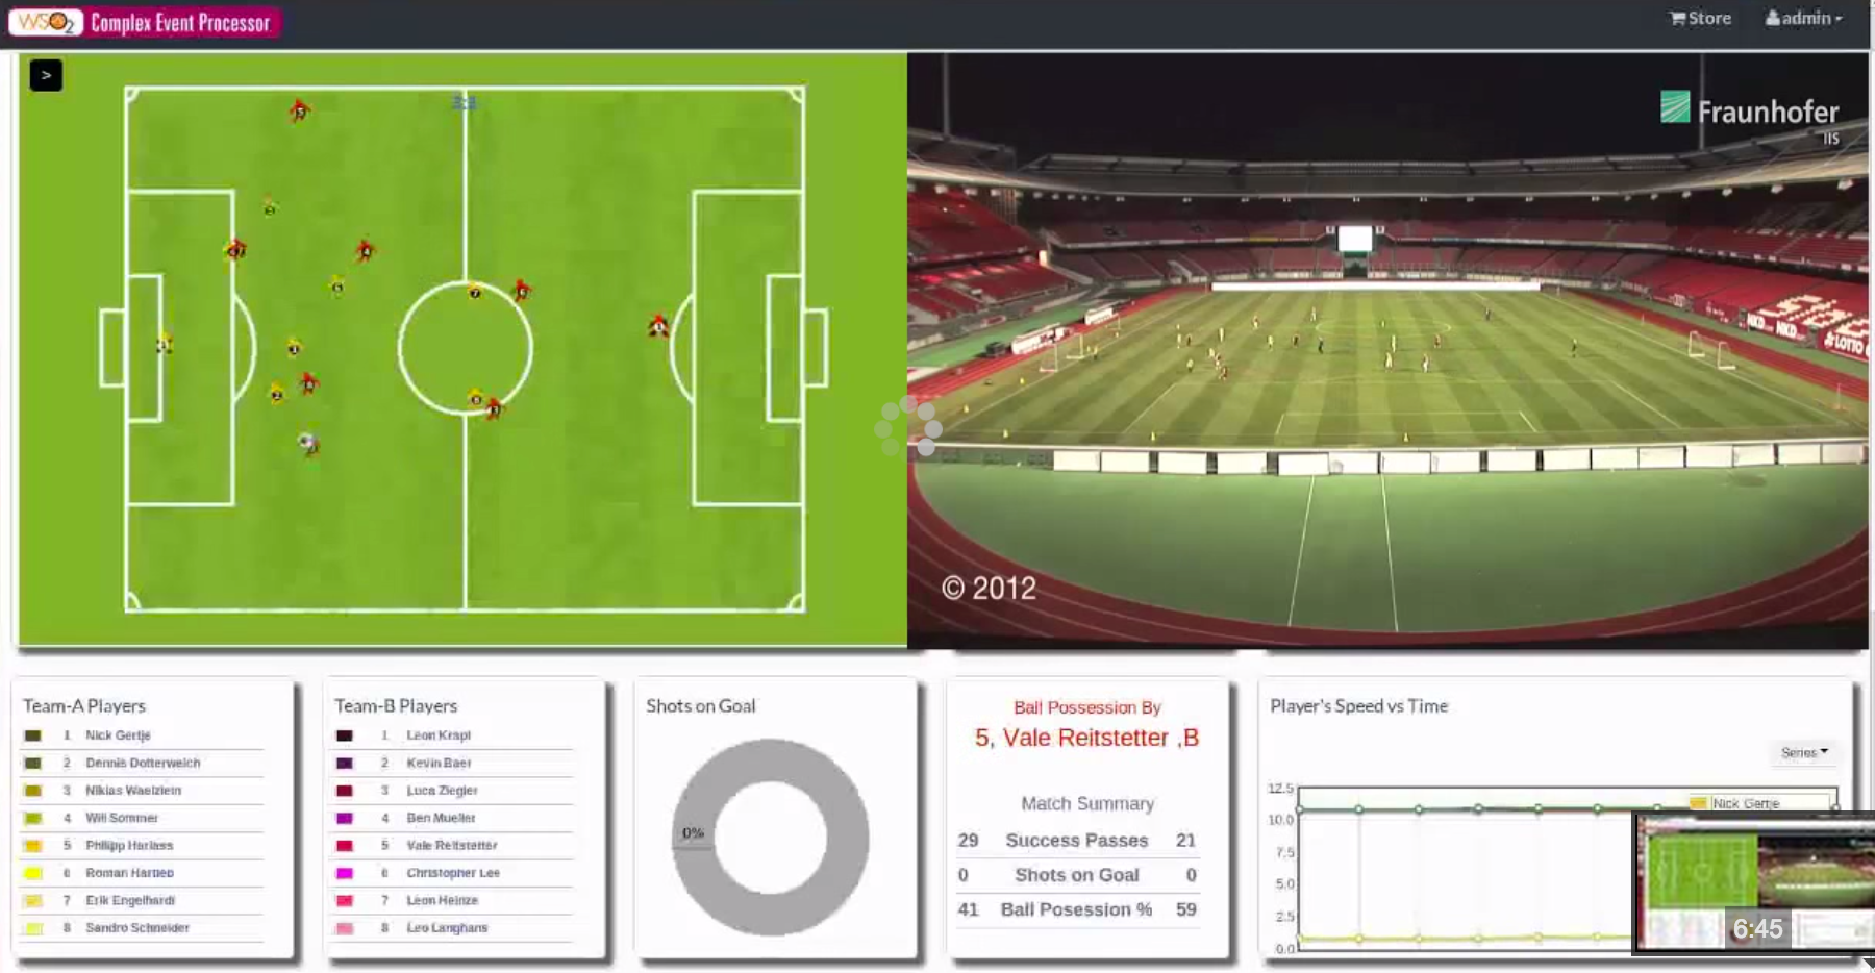
\epsfig{file=images/football.eps, height=1.5in}
\caption{Football Demo}
\label{fig:q2}
\end{figure}

In the video, we used patterns on event sequence to detect the ball possession (the time period a specific player controlled the ball). A player possessed the ball from the time he hits the ball, until someone else hits the ball. This condition can be written as a regular expression: a hit by me, followed by any number of hits by me, followed by a hit by someone else.  (We already discussed how to detect the hits on the ball in Pattern 4: Joins).  

\subsection{Pattern 8: Tracking}
The eighth pattern tracks something over space and time and detects given conditions. Following are few examples 
\begin{enumerate}
\item Tracking a fleet of vehicles, making sure that they adhere to speed limits, routes,  and geo-fences. 
\item Tracking wildlife, making sure they are alive (they will not move if they are dead) and making sure they will not go out of the reservation. 
\item Tracking airline luggage and making sure they have not been sent to wrong destinations
\item Tracking a logistic network and figuring out bottlenecks and unexpected conditions. 
\end{enumerate}

For example, TFL Demo we discussed under pattern 2 shows an application that tracks and monitors London buses using the open data feeds exposed by TFL(Transport for London). 


\subsection{Pattern 9: Detecting Trends}
We often encounter time series data. Detecting patterns from time series data and bringing them into operator attention are common use cases. 

Following are some of the examples of trends. 

\begin{enumerate}
\item Rise, Fall
\item Turn (switch from rise to a fall)
\item Outliers
\item Complex trends like ``Triple Bottom" and ``Cup and Handle"~\cite{bulkowski2011encyclopedia}.
\end{enumerate}

These trends are useful in a wide variety of use cases such as 

\begin{enumerate}
\item Stock markets and Algorithmic trading 
\item Enforcing SLA (Service Level Agreement), Auto Scaling, and Load Balancing 
\item Predictive maintenance ( e.g., guessing weather the Hard Disk will fill within the next week)   
\end{enumerate}

\subsection{Pattern 10: Running the Same Query in Batch and Realtime Pipelines}

This pattern runs the same query in both Relatime and batch pipelines. It is often used to fill the gap left in the data due to batch processing. For example, if batch processing takes 15 minutes, results would lack the data for last 15 minutes. 

Idea of this pattern, which is sometimes called ``Lambda Architecture", is to use realtime analytics to fill the gap. Nathen Marz's ``Questioning the Lambda Architecture"~\cite{lambdaQ} discusses this pattern in detail.


\subsection{Pattern 11: Detecting and Switching to Detailed Analysis}
Main idea of the pattern is to detect a condition that suggests some anomaly, and further analyze it using historical data.  This pattern is used with the use cases where we cannot analyze all the data with full detail. Instead we analyze anomalous cases in full detail. Following are few examples. 

\begin{enumerate}
\item Use basic rules to detect Fraud (e.g., large transaction), then pull out all transactions done against that credit card for larger time period (e.g., 3 months data) from batch pipeline and run a detailed analysis 
\item While monitoring weather, detect conditions like high temperature or low pressure in a given region, and then start a high resolution localized forecast on that region. 
\item Detect good customers, for example through expenditure of more than $\$1000$ within a month, and then run a detailed model to decide potential of offering a deal. 
\end{enumerate}

\subsection{Pattern 12: Using a Model} 
Idea is to train a model (often a Machine Learning model), and then use it with the Realtime pipeline to make decisions. For example, you can build a model using R, export it as PMML (Predictive Model Markup Language) and use it within your realtime pipeline. 

Following are few examples.
\begin{enumerate}
\item Fraud Detection
\item Segmentation 
\item Predict next value 
\item Predict Churn 
%TODO How about realtime machine learning ?
\end{enumerate}


\subsection{Pattern 13: Online Control} 
There are many use cases where we need to control something online. The classical use cases are autopilot, self-driving, and robotics. These would involve problems like current situation awareness, predicting next value(s), and deciding on corrective actions. 


\section{Related Work}

{\renewcommand{\arraystretch}{1.8}
\begin{table*}[htbp]
\begin{center}
\caption{Comparison With Earlier Methods}
\label{table:datasets}
\begin{tabular}{| l | c | c | c | c |}
\hline
& Coral8 patterns & Esper	& Cugola	& EPTS Reference Arch \\ \hline
Pattern 1: Preprocessing &	yes &	yes &	yes &	yes \\ \hline
Pattern 2: Alerts and Thresholds & & yes &  & \\ \hline		
Pattern 3: Simple counting and Counting with Windows & 	yes &	yes &	yes &	yes \\ \hline
Pattern 4: Joins &	yes &	yes &	yes	& yes \\ \hline
Pattern 5: Data Correlation, Missing and Erroneous Data & & yes	& yes	& yes \\ \hline
Pattern 6: Interacting with Databases & yes & & &		\\ \hline
Pattern 7: Detecting Temporal Event Sequence Patterns &	yes & yes & yes	& yes \\ \hline
Pattern 8: Tracking & & & &	yes \\ \hline
Pattern 9: Detect trends &  & yes	& &	yes \\ \hline
Pattern 10: Same Query in Batch and Realtime Pipelines & & & &\\ \hline
Pattern 11: Detecting and switching to Detailed Analysis & & & & \\ \hline
Pattern 12: Using a Model & & & &		yes \\ \hline
Pattern 13: Online Control & & & & \\ \hline
\end{tabular}
\end{center}
\end{table*}

Earlier efforts have identified common streaming realtime operators and patterns. For an instance, most Complex Event Processing technologies have adopted a SQL like query languages thus adopting operators from SQL. They, however, added more operators like windows and temporal pattern recognition to better handle the time dimension. Most such tools support patterns such as filters, transforms, windows, joins, and temporal event patterns. Cugola and Margara~\cite{cugolaprocessing} have defined a classification of these operators and done an extensive survey of different tools. However, as shown by table 1, the paper focuses on basic abstract operators as oppose to higher-level patterns. 

Technical community has also discussed this issue several times. For an example, Esper provides about 50 patterns in their solution patterns document~\cite{esperPatterns}. Although the document does not try to cover all categories, it provides insight into common problems faced by streaming query developers. Most Esper patterns are very specific and defined on narrow use cases. However, since the patterns have grown from user feedback over time, they provide a good indication of problems people trying to solve with event processing systems. 

Coral8 white paper~\cite{Coral810patterns} discusses ten patterns. As Table 1 depicts most of them matche directly to the patterns discussed in this tutorial. Among ones that did not match, we considered in-memory caching as an implementation detail of database mapping (Pattern 6). We considered hierarchical processing as a preprocessing step in generating events. Also we considered dynamic queries not as a pattern, but as an implementation detail on how query interface between users and the system is constructed. 

Event Processing Technical Society's (EPTS) reference architecture~\cite{eptsRefArch} comes very close to the patterns we discussed in this tutorial. In contrast to other efforts, the EPTS reference architecture identifies higher-level patterns such as tracking, prediction and learning in addition to low-level operators that comes from SQL like languages. Allowing for wider interpretations, EPTS patterns can contain almost all patterns we discuss. Notable exception is streaming patterns that incorporate batch processing, which is an idea developed much later. 

Patterns we introduced incorporate basic complex event processing patterns that come from SQL like languages as well as the higher-level use cases like tracking and detecting trends.  They are defined with more focus on the user rather than with the mechanics of processing implementation. For example, we called the first two patterns ``Preprocessing and Alerts" instead of calling it a filter. Following Table 1 shows how each of above approaches matches the patterns introduced in this tutorial. 

\section{Pattern Implementations}  

In this section we will discuss how the above patterns can be implemented with Apache Storm~\cite{storm} and WSO2 Complex Event Processor~\cite{siddhi}. 

Apache Storm is a distributed stream processing engine, which allows users to write queries (topologies as per Apache Storm terminology) as JavaBeans and deploy them into a cluster. It uses components named Spouts for fetching events from external systems and Bolts for processing those events. Since Spouts and Bolts are written as Java classes it allows us to implement almost any use case. In this tutorial we are omitting the implementation details of Spouts because it is same for all the use cases and depends on the transports and the protocol used for retrieving the events. 

As the Complex Event Processing Server, we will use WSO2 CEP. It accepts queries via SQL like query language and supports filters, transformations, windows, joins, temporal event patterns, and interacting with databases with data streams. At the distributed mode, WSO2 CEP can compile a given query to set of queries that run as an Apache Storm topology where each Bolt would run a WSO2 CEP engine as a Java library. We call this Java Library as Siddhi~\cite{siddhilib}.

Following is an example query supported by WSO2 CEP. 

\lstset{language=siddhi}
\begin{lstlisting}[mathescape]
from inputStockStream[price > 100]
select symbol, price * volume as transactionAmount
insert into outputStockStream
\end{lstlisting}


Similar to Apache Storm, for simplicity, we are going to omit the implementation details of event retrieval and stream management configurations with WSO2 CEP as well. 

Apache Storm based implementation of the above described patterns needs writing Java code. For brevity, we will use pseudocode to explain the implementations. 

Each Apache Storm query is specified as one or more bolts. Each bolt is represented as a method called PROCESS(E) where E is the event. E.attribute-name refers to a specific attribute of the event. Method NEW\_E() creates a new event. Also there is a special method SEND2\_NEXT\_PROCESSOR (E) that sends the event to next processor (bolt) in the topology.  We will also use few utility methods and make their function obvious by the name. Apache Storm decides next processor based on the topology. 

While explaining the WSO2 CEP based solution, we will use Siddhi Query language, which is the SQL like event query language used by WSO2 CEP. 


\subsection{Implementation of Preprocessing}

For the first pattern, lets consider a StockQuote Stream with attributes transactionAmount, symbol, price, volume, and a timeout. In this example, we filter all transactions greater than 100 and then transform the stream to output only the symbol and the last transactionAmount attributes of that stock. 

The pseudo code implementation of filtering events can be depicted as below. 


\begin{lstlisting}[mathescape, showstringspaces=false]
PROCESS(E) 
	if E.price >= 1000
		SEND2-NEXT(E); 
	END
END
\end{lstlisting}


Similarly reshaping, transforming streams, splitting and combining the attributes of a stream can be implemented as following.

\begin{lstlisting}[mathescape, showstringspaces=false]
PROCESS(E, N) 
	En = NEW_E(); 
	//transform
	En.transactionAmount = E.price*E.volume;
	En.symbol = E.symbol;
	SEND2_NEXT_PROCESSOR(En); 
 END
\end{lstlisting}


Following CEP query implements both filtering and transformations. 

\begin{lstlisting}[mathescape, showstringspaces=false]
from inputStockStream[price > 100]
select symbol, price * volume as transactionAmount
insert into outputStockStream 
\end{lstlisting}



\subsection{Implementation of Alerts and Thresholds}
This pattern can be implemented using the same techniques as filters in the first pattern. We have identified Alerts as a different pattern because the user's intent is different in the two patterns. 


\subsection{Implementing Simple Counting and Counting with Windows}
The implementation for counting can be explained by an example where we collect number of events and then calculate aggregate values based on those collected events. For an example, we can use this pattern to calculate the sum of all stock quotes last 60 seconds. 

For Storm implementation we assume a window data structure that collects data and can detect when window has expired. 

\begin{lstlisting}[mathescape, showstringspaces=false]
W = NEW WINDOW(WINDOW_TIME); 

PROCESS(E) 
	WINDOW_ADD(E.price*E.amount, E.timeStamp); 
	REMOVE_EXPIRED_EVENTS(W, E.timestamp)
	FOR v in W
		SUM = SUM + V; 
	END
	En = NEW_E(); 
	En.sumOfAmount =  SUM; 
	SEND2_NEXT_PROCESSOR(En); 
	
END
\end{lstlisting}


We can implement a counting example with CEP as follows.

\begin{lstlisting}[mathescape, showstringspaces=false]
from inputStockStream[symbol == `GOOG']#window.time(60s)
select sum(price*volume) as totalAmount
insert into lastMinStocksOfGOOG; 
\end{lstlisting}


Here we are implementing a 60 seconds batch window and we use it to generate the totalAmount of the GOOG stocks that were trading over the last hour. However, there are many other types of windows available:  sliding time windows, length batch window, length sliding window, unique window, first unique window, etc.  We will not discuss them in detail, but most Complex Event Processing engines, including WSO2 CEP, have support for those windows. 

\subsection{Implementation of Event Streams Joins}
When joining multiple streams, we can not join the current event of a particular stream against all the events that have arrived so far from the other stream. This is because it is expensive to hold all the events in memory or even at an external storage. Therefore, with realtime streaming use cases, we store only a predefined amount of events (based on time, length or via other criteria) and match against those. For a successful implementation of the join pattern, we will need a criteria for storing historic events and the ability to match the conditions against that dynamic storage. 

For this example, lets consider the football game described with the pattern where we join the ball and player streams to detect a kick. The following pseudo code explains the Storm implementation. 

For this use case, we assume there are two window implementations that can be used to retain events. 

\begin{lstlisting}[mathescape, showstringspaces=false]
BALL_W = NEW_LENGTH_WINDOW(1); 
PLAYER_W = NEW_UNIQUE_WINDOW();

PROCESS(E)
	if E instanceof  ballStream
		UPDATE_WINDOW(BALL_W, E);
		IF E.acceleration > 55
    		LIST = FIND_EVENTS(PLAYER_W, E, "I $\in$ W
    				| mod(I.position - " + E.position + " < 1");
				for Et in LIST
					SEND2_NEXT_PROCESSOR(Et);
				END	
		END
	else
		UPDATE_WINDOW(PLAYER_W, E)
		LIST = FIND_EVENTS(BALL_W, E,
			"I $\in$ W|  I.acceleration > 55
			and mod(I.position - " + E.position );
		for Et in LIST
			SEND2_NEXT_PROCESSOR(Et);
		END
	END
END  
\end{lstlisting}


 

This implementation keeps two windows, one for events from the ball stream and one for the events from player stream. Whenever, we receive an event we update the corresponding window and search for a matching event in the other window based on the given condition. Any events that matches we send forward to the next processor. 

If windows could hold a large number of events, we would need to build indexes to make FIND\_EVENTS faster. 

Following query shows the same use case implemented with Complex Event Processing.  


\begin{lstlisting}[mathescape]
from ballStream#window.length(1) 
	join palyerStream#window.unique(palyerId)
	on ballStream.acceleration > 55 
		and mod(ballStream.position - 
				palyerStream.position) < 1
select ballStream.position, palyerStream.palyerId,
insert into ballKickSteam;
\end{lstlisting}



\subsection{Implementation of Data Correlation, Missing Events and Erroneous Data}

We can implement data correlation using same techniques as Pattern 4. However, detecting missing events and erroneous data is much more complex. Here we will look at how we can implement detection of missing events in a data stream. As the example use case, we detect the customer requests that have not been responded within 1 hour of it's reception.  


\begin{lstlisting}[mathescape, showstringspaces=false]
W = NEW_SLIDING_WINDW(1h); 

PROCESS(E)  
    if E instanceof RequestEvent
       EX_LIST = PUT_AND_GET_EXPIRED_EVENTS(E, E.timeStamp);
       for En in EX_LIST
           SEND2_NEXT_PROCESSOR(En); 
			END        
    else if E instanceof ResponseEvent
       REMOVE_EVENT("e $\in$ W| E[`txID'] == e[`txID') 
    else 
       ERROR();
    END   
END 
\end{lstlisting}


Here we keep a list of requests and remove them when the request has been served (detected via ResponseEvent). If request is in the list for more than 1 hour, we raise an event after it is expired. 

CEP query for the same use case is given below. 

\begin{lstlisting}[mathescape, showstringspaces=false]
from requestStream#time.window(1 hour)
insert expired events into expiryStream;

from r1=requestStream -> 
	r2=responceStream[r1.id == id] 
	or r3=expiryStream[r1.id == id]
select r1.id as id, ...
insert into alertStream 
having r2.id == null
\end{lstlisting}



\subsection{Implementation of Databases Interactions}
We can implement Pattern 6 with storm using the code similar to Pattern 4 with calls to a database instead of storing and searching for data in-memory. Furthermore, it will only have to keep events for one stream. 

For example, lets assume we want to retrieve the customer age from a database using customer ID attribute as the key and enrich the event with customer's age. 


\begin{lstlisting}[mathescape, showstringspaces=false]
PROCESS(E) 
	RECORD = READ_FROM_DB_WITH_CACHE(
		"SELECT age FROM CUSTOMER_TABLE 
			WHERE custID = "+ E[`custID']");    
	 E.age = RECORD.age;
	 SEND2_NEXT_PROCESSOR(E); 
END   
\end{lstlisting}



In WSO2 CEP, for merging events with data in a database, or for collecting and updating them based on conditions we use a construct called Event Table. This allows Siddhi to represent historic data stored in a database as a table allowing it to be combined with active event streams at realtime. 

Let us implement the earlier use cases with CEP.

\begin{lstlisting}[mathescape, showstringspaces=false]
define table CustomerTable (customerId string, 
	customerName string, customerAge int);

from TxStream join CustomerTable
	on TxStream.userId == CustomerTable.customerId
select userId as id, CustomerTable.customerAge as age, 
insert into fraudDetectionStream
\end{lstlisting} 

Here event table matches data in a database to a window, and we can join against the window as any window.

\subsection{Implementation of Temporal Event Sequences and Patterns}

Implementing sequences and patterns with Storm is complex. Hence let us look at a simple  fraud detection use case where we detect a small transaction (amount less than \$50) from a credit card followed by a very large transaction (amount larger than \$10000) from the same card within a day. 

The pseudo code explaining the scenario implementation is as follows.
 
\begin{lstlisting}[mathescape,showstringspaces=false]
M = NEW_MAP()

PROCESS(E)  
	KEY = CONCAT(E.cardNumber); 
	if E.amount < 50
		MAP_PUT(M, KEY , E.amount); 
	else If E.amount > 10000
		if MAP_CONTAINS(M, KEY)
			MAP_REMOVE(M, KEY));
			//send the event		     
			SEND2_NEXT_PROCESSOR(E); 
		END
	else
		ERROR();
	END	
END
\end{lstlisting}  
 

Above code detects two events that follow each other. In the general case, the pattern can be expressed as a regular expression and the system needs to simulate a state machine to implement them. Moreover, the system needs to expire events to avoid pattern collecting all small transaction events and running out of memory. We will not discuss the implementation of these details in this paper. 

At the meantime  temporal sequences and patterns can be easily implemented in CEP systems as they are provided as out of the box constructs. The following segment of Siddhi query explains the above scenario.


\begin{lstlisting}[mathescape, showstringspaces=false]
from a1 = transactionStream[amount < 50 ] -> 
        a2 = transactionStream[a1.cardNo == cardNo 
        	and amount > 10000]
        within 1 day
select a1.cardNo as cardNo, a1.amount as firstAmmount, 
	a2.amount as currentAmount, ...
insert into fraudDetectionStream
\end{lstlisting} 

Here `->' denotes `followed by', meaning after the first event its corresponding next event can appear after any number of other events. 


\subsection{Implementation of Trend Detection}

Detecting trends is one of the key streaming analytics use cases. Trends are widely used in both Stock markets and algorithmic trading. For example, stock market traders have identified chart patterns like Triple Bottom pattern~\cite{bulkowski2011encyclopedia} that are significant behaviors in the market that are actionable. 

Identifying even basic trends like a peak require us to implement a state machine depicted in Figure~\ref{fig:q4}. We will not implement this use case with Storm as it is complicated. 

\begin{figure}[!htbp]
\centering
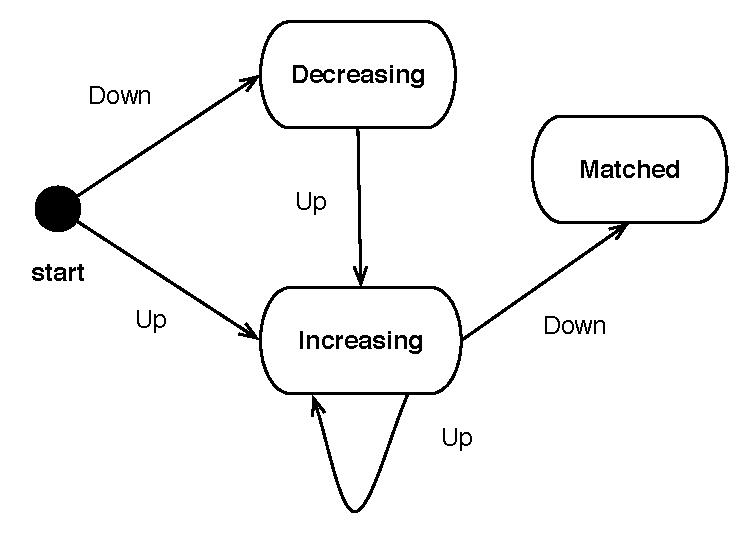
\epsfig{file=images/peakState.eps, height=1.5in}
\caption{State Machine to Detect a Peak}
\label{fig:q4}
\end{figure}

However, if we ignore the noise, we can easily detect most trends as temporal event patterns using CEP. For example, the following query identifies a peak in GOOG stock price. 


\begin{lstlisting}[mathescape, showstringspaces=false]
from stockStream[symbol=='GOOG'] 
insert into googStockStream

from a1=googStockStream, 
        a2=googStockStream[last.price<=price]+,
        a3=googStockStream[a2.price>price]
select a2[last].price as peekPrice, 
	a3.price as currentPrice
\end{lstlisting} 

If we need to process the above for all the symbols independently, then we have to partition the stockStream and process the events in parallel and this can be implemented as below.

\begin{lstlisting}[mathescape, showstringspaces=false]
partition with ( symbol of stockStream)
begin 
    from a1=strockStream, 
            a2=strockStream[last.price<=price]+,
            a3=strockStream[a2.price>price]
    select a2[last].price as peekPrice, 
    	a3.price as currentPrice
end;
\end{lstlisting} 

However, a real life trend detection needs to be resilient against the noise. For an example, Rashmi Arachchi et al.~\cite{chartPatterns} used kernel regression to detect maxima and minimas and then applied temporal events patterns to those maximas and minimas to identify high-level chart patterns. 

\subsection{Implementing the Same Query in Batch and Realtime pipelines}

This pattern is often implemented combining a batch-processing tool like MapReduce and a realtime processing tool like CEP. As shown by Figure~\ref{fig:q3}, the main idea is to periodically run the batch processing code and place the results in a database. Then we combine the results from the batch process that is in the database or a distributed cache using Pattern 6: Merge with data in a database. 

\begin{figure}[!htbp]
\centering
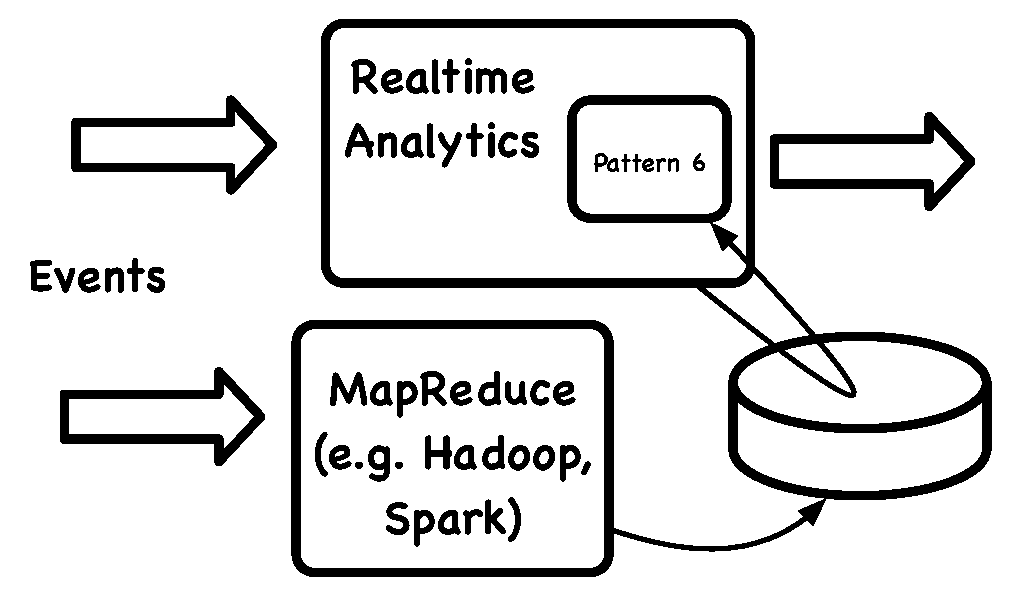
\epsfig{file=images/lambda.eps, height=1.5in}
\caption{Lambda Architecture}
\label{fig:q3}
\end{figure}

%For an example, lets assume that we are trying to find the quote with the maximum value in a stock quote stream. We write data to a database and MapReduce system process that data and write them to historicDataTable. 

%Following code shows a naive implementation of this pattern using CEP Queries. 

%\begin{lstlisting}[mathescape, showstringspaces=false]
%@from(.. backed by database ..)
%define table historicDataTable (id string, double maxValue...);

%from StockQuoteStream join historicDataTable
%	on StockQuoteStream.amount 
%insert into historicDataTable;

%from batchResultsStream 
%delete temporalDataTable
%	on batchResultsStream.timestamp 
%		> temporalDataTable.timestamp;

%from inputStream
%insert into temporalDataTable; 

%from requestStream  join temporalDataTable
%	on requestStream.id==temporalDataTable.id
%insert into responseStream

%from requestStream  join historicDataTable
%	on requestStream.id==temporalDataTable.id
%insert into responseStream
%\end{lstlisting} 

%A similar implementation is also possible with Apache Storm using the method described in Pattern 6: Merge with data in a database.


\subsection{Implementation of Detecting a condition and Switching to Detailed Analysis}
For an example, we can detect fraudulent conditions using a realtime engine in streaming fashion and then trigger a detailed analysis with a batch processing engine like MapReduce. As shown by Figure\ref{fig:q4}, we can implement this pattern by first using Alert, Event Sequences, Trends patterns to detect the condition and then triggering a batch job using a MapReduce cluster. 

\begin{figure}[!htbp]
\centering
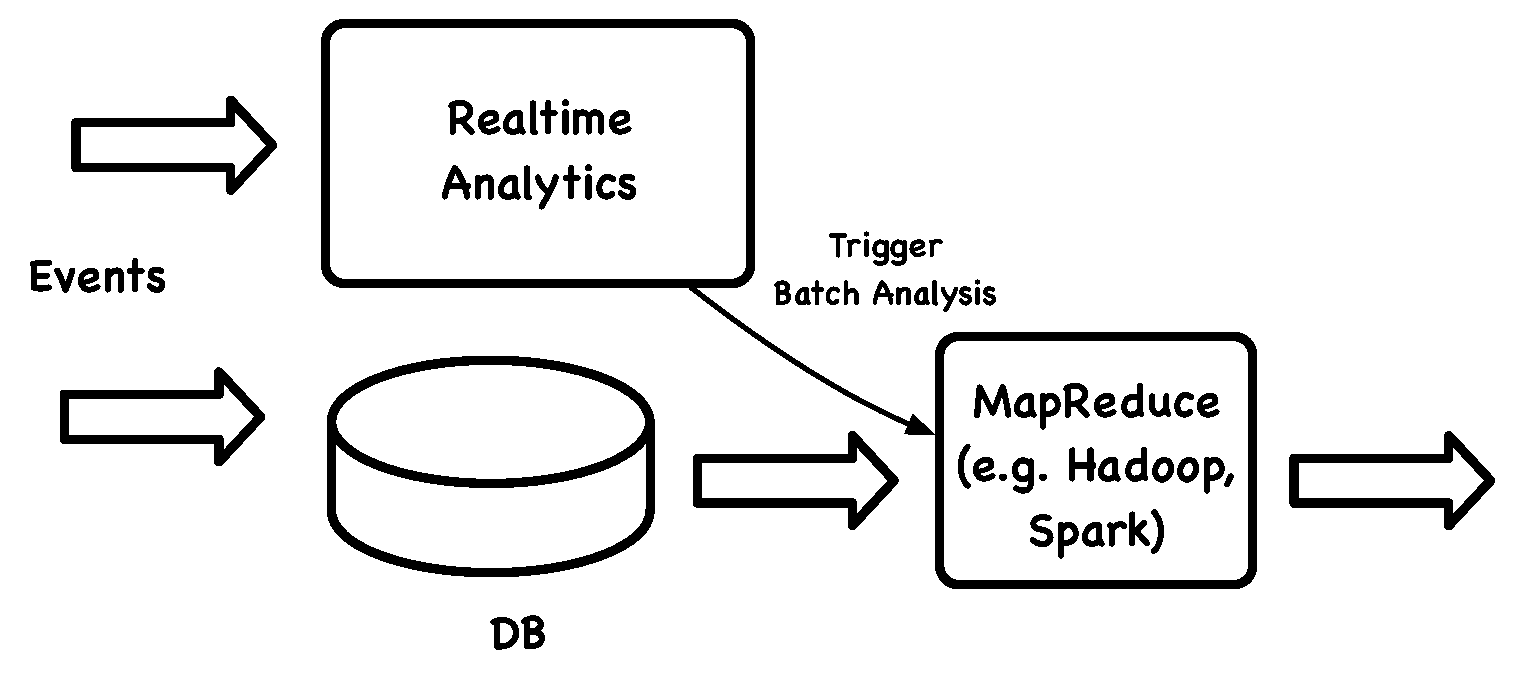
\epsfig{file=images/detailAnalysis.eps, height=1.5in}
\caption{Trigger Batch from Realtime}
\label{fig:q4}
\end{figure}

For example, we have built a credit card fraud detection solution that detects suspicious activities and lets a human operator explore related data for more information. For example, when the system flags a credit card transaction as suspicious, the operator can pull out all other transactions done by the same card and make a final decision. Instead by having a human int the loop, the system can also trigger a detailed analysis. 


%TODO more details about Fraud solutions 

\subsection{Implementation of Using a Model}

The idea is to use a Machine Learning model built elsewhere within realtime analytic processing. For example, we can use R language to build a model (e.g., logistic regression model) and then export the model as a Predictive Model Markup Language (PMML) Model. We can run the PMML model from WSO2 CEP using it's PMML extension. Similarly, we can use PMML interpreter like JPMML within a Storm Bolt to implement a similar solution. 

A sample query of running machine learning model in WSO2 CEP is as follows.


\begin{lstlisting}[mathescape, showstringspaces=false]
from TrasnactionStream
	#ml:applyModel(`/path/logisticRegressionModel1.xml',  
		time stamp, amount, ip) 
insert into PotentialFraudsStream;
\end{lstlisting} 

\subsection{Implementation of Online Control} 

For example, lets consider keeping a car's speed close to a given limit. This can be implemented by using a pattern we discussed before to detect the conditions and then carry out an action to control the car. 

For an example, if we need to keep the car's speed in 50 kmph, we can have one query that detects when it is over 55 kmph and apply breaks, and another that detects when it is less than 45 kmph and accelerate the car. Both above queries can be implemented with Alerts Pattern. 

However, real life implementations of online control is much more complicated due to factors like it takes time for operations to take effect and we need to wait for one operation to finish before issuing another one. Furthermore, certain conditions might lead to oscillations. For example, a car that repeatedly accelerates and decelerates is not very comfortable to ride on. We will not explore those details in this discussion. 

\section{Conclusion} 

Although there is much interest in realtime analytics, much focus is on counting use cases. Despite being useful, such use cases are only a small portion of realtime analytics use cases. Since the input data arrives as a data stream, a time dimension always presents in the data. This time dimension allows us to implement and perform much powerful use cases.  

Most current tools forces every programmer to design and implement realtime analytics processing from first principles. For an example, if users need a time window, they need to implement it from first principals.  This is like every programmer implementing his own list data structure. Better understanding of common patterns will let us understand the domain better and build tools that handle those scenarios. This tutorial tried to address this gap by describing thirteen common relatime analytics patterns and how to implement them. Furthermore, we discussed several real life use cases where those patterns are useful.


%
% The following two commands are all you need in the
% initial runs of your .tex file to
% produce the bibliography for the citations in your paper.
\bibliographystyle{abbrv}
\bibliography{sigproc}  % sigproc.bib is the name of the Bibliography in this case
% You must have a proper ".bib" file
%  and remember to run:
% latex bibtex latex latex
% to resolve all references
%
% ACM needs 'a single self-contained file'!
%
%APPENDICES are optional
\end{document}
